\documentclass[11pt]{article}

\newcommand{\squishlist}{
   \begin{list}{$\bullet$}
    { \setlength{\itemsep}{0pt}      \setlength{\parsep}{3pt}
      \setlength{\topsep}{3pt}       \setlength{\partopsep}{0pt}
      \setlength{\leftmargin}{1.5em} \setlength{\labelwidth}{1em}
      \setlength{\labelsep}{0.5em} } }

\newcommand{\squishend}{
    \end{list}  }

\usepackage{times}
\usepackage{mathptm}
\usepackage{fullpage}
\usepackage{graphicx}
 
\begin{document}

\begin{center}
{\bf{Regis University -- Physics 305A -- Fall 2019 -- Lab 9: Friction}} 
\end{center}

\noindent You have talked about friction forces in general terms.  In today's lab, we will study them quantitatively.  Friction forces oppose the sliding motion of two surfaces that are in 
contact with each other.  The more firmly the surfaces are
pressed together, the larger the friction forces are.  We can capture 
this relationship in an equation: $F_f = \mu F_N$: the friction force is
proportional to the normal force, with a proportionality constant known 
as a ``coefficient of friction'' and represented by the Greek 
letter $\mu$ (mu).  A small value of $\mu$ indicates that the surfaces 
are slippery, and a large value indicates that they are rough or sticky.
For example, Teflon-on-Teflon has $\mu \approx 0.04$, while wood-on-wood 
might fall somewhere between 0.3 and 0.5, depending on the details.

In fact, we can further divide friction forces into two categories: static 
and kinetic.  If the two surfaces are sliding on each other, then {\em kinetic}
friction applies, and $F_{KF} = \mu_k F_N$.  If they are not (yet) sliding
on each other, then {\em static} friction prevents them from starting to slide,
with $F_{SF} \le \mu_s F_N$.  The ``less than or equal to'' sign indicates 
that the static friction force may not need to be that large to prevent
sliding -- it will only be as large as it needs to be, up to the limit 
set by $\mu_s F_N$.   For most kinds of surfaces, $\mu_s > \mu_k$, which 
implies that more force is required to start an object sliding than to 
keep it sliding after it has started.  

\section{Measuring coefficients of friction}

In the first part, you can use a Vernier force sensor to pull a block of wood 
across the table with varying amounts of weight stacked on top:

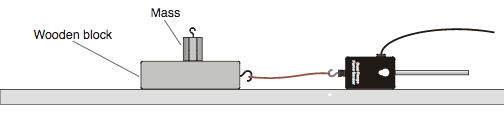
\includegraphics[width=0.7\textwidth]{FrictionBlock.png}

From a graph of $F$ vs. time, you should be able to identify the 
maximum static friction force (at a time just before the block moves) and the 
kinetic friction force.  You can plot graphs of $F_{SF}$ versus $F_N$ and
$F_{KF}$ vs. $F_N$ to determine $\mu_s$ and $\mu_k$.  Please use a program
such as Logger Pro (rather than Excel) to fit lines to these graphs so that 
you can determine the {\em uncertainty} in your measurement of each coefficient.


\section{Measuring acceleration of the block}

Start by making a prediction, based on your results from the previous section:
if you give your block of wood (without any weights on 
  top) a push so that it slides across the table, what will its acceleration be as it gradually comes to a stop?  

Now, do the experiment, using a Vernier motion detector to track the 
position, velocity, and acceleration of the block.  You will need to be 
careful to slide the block in a way that it goes straight and does not
rotate; this will take some practice.

Take at least 5 ``good'' runs (where there is no obvious rotation) 
and record the acceleration for each run.  Compute the average (mean) value
for the acceleration and its uncertainty (remember $\sigma / \sqrt{N}$,
where $\sigma$ is the standard deviation).  

Does this value agree, within a reasonable multiple of your calculated 
uncertainty, with your original prediction?


\end{document}
